%versi 2 (8-10-2016)
\chapter{Landasan Teori}
\label{chap:landasanteori}
Bab ini akan membahas landasan teori yang dipakai dalam pembangunan proyek ini. Pembahasan akan mencakup \textit{framework} yang digunakan, teori \textit{web service}, protokol HTTP dan pengenalan API.

\section{Framework Codeigniter}
\label{sec:codeigniter} 

Pembangunan proyek ini akan menggunakan \textit{framework Codeigniter} yang akan disingkat menjadi CI kedepannya. CI adalah \textit{framework} atau sebuah \textit{toolkit} yang membantu pengembangan aplikasi web menggunakan PHP. Tujuan dari CI adalah mempercepat pengembangan proyek dibanding jika membuat semuanya dari awal. CI menyediakan \textit{library} yang bisa dimanfaatkan untuk kebutuhan-kebutuhan umum. CI mengizinkan pengguna untuk lebih fokus ke inti dari proyeknya dengan meminimalisir jumlah kode yang dibutuhkan untuk hal tertentu. ~\cite{ellisLab:20:codeIgniter1}

CI adalah \textit{framework} gratis di bawah lisensi MIT. CI merupakan \textit{framework} yang cepat dan ringan dibandingkan dengan \textit{framework} lainnya. Ini dikarenakan sistem inti dari CI yang hanya membutuhkan \textit{library} yang sangat sedikit. \textit{URL} yang dibuat oleh CI cukup sederhana dan mudah digunakan di \textit{search engine}.

CI memiliki alur data seperti berikut:

\begin{figure}[H]
\center
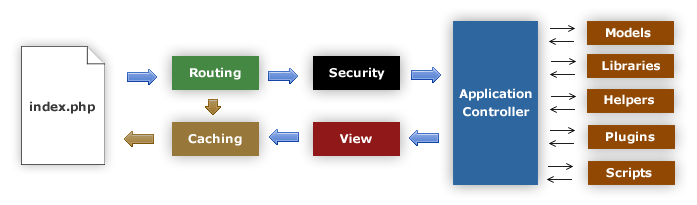
\includegraphics[width=\textwidth,height=\textheight,keepaspectratio]{Gambar/codeigniterflow.png}
\caption{Aliran Data CI. ~\cite{ellisLab:20:codeIgniter2}}
    \label{img:CIdataflow}
\end{figure}

Gambar ~\ref{img:CIdataflow} dapat dijelaskan sebagai berikut:
\begin{enumerate}
	\item File index.php berfungsi sebagai \textit{controller} utama yang menginialisasi \textit{resources} yang dibutuhkan untuk menjalankan CodeIgniter.
	\item \textit{Routing} memeriksa permintaan HTTP untuk menentukan apa yang harus dilakukan.
	\item Jika \textit{file cache} sudah ada, \textit{file} tersebut langsung dikirim ke \textit{browser}, menerobos eksekusi sistem normal.
	\item Jika \textit{cache} tidak ditemukan, permintaan akan diteruskan ke \textit{Security}. Sebelum \textit{controller} akan dimuat, permintaan HTTP dan data yang dikirim oleh pengguna akan disaring untuk keamanan.
	\item Setelah itu di \textit{controller} akan memuat model, \textit{library} penting, \textit{helpers}, dan \textit{resources} lain yang dibutuhkan untuk memproses permintaan spesifik.
	\item Tampilan akhir dimuat dan dikirim ke \textit{browser} untuk dilihat. Jika \textit{cache} diaktifkan, tampilan akan di-\textit{cache} terlebih dahulu sehingga jika ada permintaan yang sama berikutnya, permintaan dapat langsung dimuat.
\end{enumerate}

CI menggunakan pola pengembangan \textit{Model-View-Controller} yang akan disingkat menjadi MVC. MVC adalah pendekatan perangkat lunak yang memisahkan logika aplikasi dari tampilan. Pada praktiknya, ini memungkinkan halaman web mengandung \textit{scripting} minimal karena tampilan akan terpisah dari \textit{scripting} PHP.
\begin{itemize}
	\item \textbf{Model} merepresentasikan struktur data. Kelas \textit{model} yang dibuat akan memiliki fungsi yang akan menolong pengguna untuk membaca, membuat, dan mengubah informasi di database.
	\item \textbf{View} adalah informasi yang akan ditampilkan pada pengguna. Halaman \textit{view} pada umumnya adalah halaman web, tapi pada CodeIgniter, \textit{view} bisa juga merupakan potongan bagian seperti \textit{header} atau \textit{footer} pada halaman web.
	\item \textbf{Controller} adalah perantara antara \textit{model}, \textit{view}, dan \textit{resources} lainnya yang dibutuhkan untuk memproses permintaan HTTP dan menghasilkan suatu halaman web.
\end{itemize}

\section{Protokol HTTP}
\label{sec:httpprotocol}

HTTP adalah sebuah protokol yang memungkinkan pengambilan \textit{resource} seperti dokumen HTML. HTTP merupakan fondasi pertukaran data di web. Protokol HTTP berbentuk \textit{client-server} yang berarti permintaan diminta oleh \textit{browser}. \textit{Server} dan \textit{client} berkomunikasi dengan saling bertukar pesan. Pesan yang dikirimkan oleh \textit{client} disebut \textit{request} dan jawaban dari \textit{server} disebut \textit{response}.

\textit{Client} dalam protokol \textit{client-server} secara umum adalah \textit{browser}. Entitas yang memulai \textit{request} dalam protokol ini pasti adalah \textit{browser}. Untuk menampilkan sebuah halaman web, \textit{browser} perlu mengirim \textit{request} untuk mendapatkan dokumen HTML yang merepresentasikan halaman. \textit{File} kemudian diproses mulai dari \textit{script}, tampilan (CSS) dan \textit{resource} lainnya seperti gambar dan video. Web \textit{browser} kemudian akan menggabungkan hasil proses tersebut untuk menampilkan halaman web.

Halaman web adalah \textit{hypertext document}. \textit{Hypertext document} mungkin memiliki beberapa teks yang merupakan sebuah link dan dapat diklik untuk membuka halaman baru. Hal ini mengizinkan pengguna untuk menjelajah web dengan mudah. \textit{Browser} menerjemahkan perintah-perintah ini dengan \textit{HTTP requests} dan mengolah \textit{HTTP responses} lebih dalam untuk memberikan respon yang lebih jelas untuk pengguna.

Di sisi lain, ada \textit{server} yang menjawab \textit{request} dari \textit{client}. \textit{Server} memberikan dokumen yang diminta sesuai permintaan \textit{client}. Sebuah \textit{server} tampak seperti sebuah mesin tapi mungkin saja sebuah \textit{server} adalah kumpulan dari berbagai \textit{server} lain yang berbagi-bagi tugas dalam membuat dokumen saat diminta. ~\cite{mozilla:19:http}

\section{Web Service}
\label{sec:webservice}

\textit{Web service} adalah layanan berbasis internet atau jaringan pribadi (intranet). \textit{Web service} menggunakan XML yang sudah distandarisasi untuk berkomunikasi. XML adalah bahasa \textit{markup} yang digunakan untuk meng-\textit{encode} dokuken dengan format tertentu sehingga dapat dibaca manusia dan mesin. Perangkat lunak ini tidak terikat sistem operasi atau bahasa pemrograman tertentu. Layanan ini memungkinkan aplikasi untuk berinteraksi dengan aplikasi lain secara langsung lewat internet.

Komponen dari \textit{web service} adalah:

\begin{enumerate}
    \item SOAP \textit{(Simple Object Access Protocol)} yang bertugas untuk meng-\textit{encode} pesan dalam format XML.
    \item UDDI \textit{Universal Description, Discovery and Integration)} yang bertugas untuk memusatkan layanan-layanan dan menyediakan fungsionalitas mudah ditemukan.
    \item WSDL \textit{(Web Services Description Language)} bertanggung jawab untuk mendeskripsikan antarmuka yang bersifat umum ke \textit{web service} spesifik.
\end{enumerate}

Web service memungkinkan komunikasi antar aplikasi dengan menggunakan XML untuk memberikan \textit{tag} kepada data, SOAP untuk mengirim pesan dan WSDL untuk menjelaskan ketersediaan layanan. ~\cite{cardoso:06:webservice}

\section{GDS API}
\label{sec:gdsapi} 

GDS merupakan akronim dari \textit{Global Distribution System}. GDS adalah sistem jaringan yang memungkinkan industri perjalanan melakukan transaksi antara satu sama lain. GDS secara umum digunakan di penerbangan, perhotelan, penyewaan mobil dan lain-lain.

Proyek situs pemesanan tiket kereta api ini menggunakan \textit{API} layanan berbasis web keagenan tiket kereta api reguler. Untuk menggunakan \textit{API} ini, pengguna harus menggunakan token yang bisa didapat dari \textit{dashboard} aplikasi GDS.

Untuk mendapatkan token, pengguna harus menambahkan \textit{IP Address} yang digunakan untuk membangun web dengan langkah-langkah sebagai berikut:

\begin{enumerate}
    \item Login ke \textit{dashboard} KDS.
    \item Pilih menu admin kemudian ke \textit{Edit User}.
    \item Pilih \textit{tab API Access}. Masukkan \textit{IP Address} yang digunakan untuk membangun web. 
    \item Tekan \textit{submit}.
    \item Token akan dibuat secara otomatis. 
\end{enumerate}

Semua modul dalam \textit{API} ini membutuhkan token untuk berjalan. Token yang salah akan selalu memberikan respon \textit{error} dari \textit{API} dengan \textit{err\_num} 001003 dan \textit{err\_str} \textit{No Access Token}. \textit{Err\_num} adalah kode numerik dari eror dan \textit{err\_str} adalah penjelasan dari eror tersebut. Keduanya akan ada di setiap respon dari \textit{API} untuk menunjukkan terjadinya eror atau tidak saat mengirimkan permintaan.

Modul dari GDS kereta api berjumlah 8 dengan nama fungsi sebagai berikut:

\begin{enumerate}
	\item data/get-station-new
	\item information/get-rail-schedule-new
	\item information/get-booking-info-new
	\item information/get-rail-seatmap-new
	\item transaction/booking-rail-new
	\item transaction/rail-change-seat-new
	\item transaction/cancel-book-new
	\item transaction/payment-new

\end{enumerate}

Ada 3 jenis modul dari GDS sesuai dengan 8 fungsi yang sudah tertera. Jenis modul-modul tersebut adalah \textit{data}, \textit{information} dan \textit{transaction}. \textit{Data} adalah jenis modul untuk mendapatkan data yang tidak membutuhkan \textit{input}. \textit{Information} adalah jenis modul untuk mendapatkan informasi dengan \textit{input} tertentu. \textit{Transaction} adalah jenis modul yang akan dicatat di \textit{server} baik itu pemesanan atau pembayaran.

\subsection{Get Station}
\label{subsec:getstation}

Modul pertama adalah \textit{data/get-station-new}. Tujuan dari modul ini adalah mendapatkan nama-nama stasiun di Indonesia beserta kodenya. \textit{Get Station} merupakan tipe \textit{data} yang tidak memerlukan parameter \textit{input}. Seperti yang dapat dilihat pada tabel \ref{tab:getstationinput}, modul ini tidak membutuhkan \textit{input} apa-apa untuk menampilkan hasilnya. Oleh karena itu respon dari modul ini akan selalu menghasilkan eror dengan kode 0 yang berarti berhasil.

\begin{table}[H]
	\centering 
	\caption{Tabel Parameter \textit{Input} untuk Modul \textit{data/get-station-new}}
	\label{tab:getstationinput}
	\begin{tabular}{|l|l|l|l|}
		\hline
		Field & Data Type & Mandatory & Description\\
		\hline
		
	\end{tabular} 
\end{table}

Hasil keluaran dari modul ini adalah \textit{array} stasiun kereta api seperti yang dapat dilihat pada tabel \ref{tab:getstationoutput}. Isi dari \textit{array result} adalah data stasiun keberangkatan dan stasiun tiba. Bentuk data stasiunnya sendiri dalah \textit{array} dengan isi kode dan nama stasiun.

\begin{table}[H]
	\centering 
	\caption{Tabel \textit{Output} untuk Modul \textit{data/get-station-new}}
	\label{tab:getstationoutput}
	\begin{tabular}{|l|l|p{8cm}|}
		\hline
		Field & Data Type & Description\\
		\hline

		\hline
        err\_num & String & Kode numerik\\
        \hline
        err\_str & String & Kode dalam string\\
        \hline
        result & Array & \{*origin, *destination\}\\
        \hline
        \hline
        *origin & Array & [\{**code, **name\}]\\
        \hline
        *destination & Array & [\{**code, **name\}]\\
        \hline
        **code & String & Kode stasiun\\
        \hline
        **name & String & Nama stasiun\\
        \hline
		
	\end{tabular} 
\end{table}


Isi dari hasil respon modul ini cukup panjang tapi mudah untuk dibaca. Contoh hasil dari modul ini adalah:

\begin{lstlisting}[language=json]
    {
        "err_num": "0",
        "err_str": "OK",
        "result": {
            "origin": [
                {
                    "code": "KTG",
                    "name": "KETAPANG"
                },
                {
                    "code": "TRK",
                    "name": "TARIK"
                },
                {
                    "code": "SB",
                    "name": "SURABAYA KOTA"
                },
                ...
                {
                    "code": "KAC",
                    "name": "KIARACONDONG"
                }
            ],
            "destination": [
                {
                    "code": "KTG",
                    "name": "KETAPANG"
                },
                {
                    "code": "TRK",
                    "name": "TARIK"
                },
                ...
                {
                    "code": "KAC",
                    "name": "KIARACONDONG"
                }
            ]
        }
    }
\end{lstlisting}

\subsection{Get Rail Schedule}
\label{subsec:getrailschedule}

Modul kedua adalah \textit{information/get-rail-schedule-new}. Modul ini mendapatkan jadwal kereta api sesuai dengan \textit{input} yang diberikan. Modul ini memiliki \textit{input} stasiun, tanggal keberangkatan dan jumlah penumpang. Hasil keluaran dari modul ini adalah jadwal-jadwal kereta api sesuai dengan \textit{input} yang diberikan.

\begin{table}[H]
	\centering 
	\caption{Tabel Parameter \textit{Input} untuk Modul \textit{information/get-rail-schedule-new}}
	\label{tab:getrailscheduleinput}
	\begin{tabular}{|l|l|l|l|}
		\hline
		Field & Data Type & Mandatory & Description\\
		\hline
		
		\hline
        org & String & YES & Kode stasiun keberangkatan\\
        \hline
        des & String & YES & Kode stasiun kedatangan\\
        \hline
        departure\_date & Date & YES & Tanggal keberangkatan (dd/mm/yyyy)\\
        \hline
        adult\_quantity & Number & YES & Jumlah \textit{adult} yang ingin memesan\\
        \hline
        infant\_quantity & Number & YES & Jumlah \textit{infant} yang ingin memesan\\
        \hline
	\end{tabular} 
\end{table}

Tabel \ref{tab:getrailscheduleinput} menunjukkan input apa saja yang dibutuhkan oleh \textit{information/get-rail-schedule-new}. \textit{Input} pertama adalah \textit{org} yang merupakan singkatan \textit{origin} dan merepresentasikan kode stasiun keberangkatan. \textit{Input} kedua adalah \textit{des} atau \textit{destination} yang merepresentasikan kode stasiun tujuan. Kemudian, modul ini juga menerima \textit{departure\_date} yang merupakan tanggal berangkat kereta. Karena modul ini hanya menerima 1 tanggal keberangkatan, maka untuk perjalanan 2 arah, modul ini harus dipanggil 2x. Parameter terakhir adalah jumlah penumpang dewasa yaitu \textit{adult\_quantity} dan bayi dengan nama parameter \textit{infant\_quantity}. Sesuai dengan aturan kereta api, yang dianggap bayi adalah penumpang dengan umur di bawah 3 tahun. Jumlah bayi tidak wajib ada untuk memesan tiket kereta api.\\

Berikut adalah contoh \textit{input} untuk modul ini:

\begin{lstlisting}[language=json]
    {
        "token":"D238681D-78A6-4EB6-BB10-1CAD13C4AEE5",
        "org":"GMR",
        "des":"BD",
        "departure_date":"30/06/2019",
        "adult_quantity":"1"
    }
\end{lstlisting}

\begin{table}[H]
	\centering 
	\caption{Tabel \textit{Output} untuk Modul \textit{information/get-rail=schedule-new}}
	\label{tab:getrailscheduleoutput}
	\begin{tabular}{|l|l|p{8cm}|}
		\hline
		Field & Data Type & Description\\
		\hline

		\hline
        err\_num & String & Kode numerik\\
        \hline
        err\_str & String & Kode dalam string\\
        \hline
        result & Array & \{*schedule\}\\
        \hline
        \hline
        *schedule & Array & [\{*org, *des, *vendor, *dep\_datetime, *arv\_datetime, *class, *transporter\_no, *subclass, *adult\_fare, *adult\_discount, *infant\_fare, *infant\_discount, *avb, *exceed\_booking\_time, *vendor\_id\}]\\
        \hline
        *org & String & Tempat keberangkatan\\
        \hline
        *des & String & Tempat kedatangan\\
        \hline
        *vendor & String & Vendor dari \textit{transporter}\\
        \hline
        *dep\_datetime & String & Waktu keberangkatan (dd/mm/yyyy-hh:mm)\\
        \hline
        *arv\_datetime & String & Waktu kedatangan (dd/mm/yyyy-hh:mm)\\
        \hline
        *class & String & \textit{Class} dari kereta api (\textit{Economy, Business, Executive})\\
        \hline
        *transporter\_no & String & Nomor kereta api\\
        \hline
        *transporter\_name & String & Nama kereta api\\
        \hline
        *subclass & String & \textit{Subclass} kereta api\\
        \hline
        *adult\_fare & String & Harga \textit{adult}\\
        \hline
        *adult\_discount & String & Harga \textit{adult} setelah diskon\\
        \hline
        *infant\_fare & String & Harga \textit{infant}\\
        \hline
        *infant\_discount & String & Harga \textit{infant} setelah diskon\\
        \hline
        *avb & String & \textit{Availability} yang tersedia\\
        \hline
        *exceed\_booking\_time & String & Variabel penanda apabila jadwal sudah melewati batas penjualan atau belum (1 berarti sudah lewati batas penjualan, 0 berarti belum)\\
        \hline
        *vendor\_id & String & Id Vendor: 1 = KAI, 2 = KAI V2\\
        \hline
		
	\end{tabular} 
\end{table}

Tabel \ref{tab:getrailscheduleoutput} menunjukkan keluaran dari modul ini. Hasil dari modul ini adalah sebuah \textit{array result} yang berisikan jadwal-jadwal kereta yang tersedia. Seperti pada \textit{input}, \textit{org} adalah stasiun keberangkatan dan \textit{des} adalah stasiun tujuan. \textit{Vendor} adalah vendor dari kereta api. Keluaran \textit{dep\_datetime} dan \textit{arv\_datetime} masing-masing adalah waktu keberangkatan dan waktu kereta tiba di tujuan. 

\textit{Class} adalah kelas dari kereta seperti ekonomi, bisnis, eksekutif dan lain-lain. \textit{Transporter\_no} adalah nomor kereta api sementara \textit{transporter\_name} adalah nama dari kereta api. \textit{Subclass} adalah sub-kelas dari kereta api dengan contoh A, B, C. Sub-kelas biasa ditentukan dari posisi tempat duduk. Tempat duduk yang strategis (dekat pintu keluar atau sebelah jendela) pada umumnya adalah A. 

\textit{Adult\_fare} adalah harga tiket untuk dewasa sementara \textit{adult\_discount} adalah harga tiket untuk dewasa setelah dipotong diskon. Hal yang sama ada juga untuk bayi dengan \textit{infant\_fare} sebagai harga tiket bayi dan \textit{infant\_discount} sebagai harga tiket bayi setelah dipotong diskon. \textit{Avb} adalah sisa jumlah kursi yang tersisa. \textit{Exceed\_booking\_time} adalah penanda apakah masih bisa melakukan booking untuk jadwal kereta tersebut. \textit{Vendor\_id} merupakan ID untuk vendor.\\

Contoh keluaran dari modul ini adalah sebagai berikut:

\begin{lstlisting}[language=json]
    {
        "err_num": "0",
        "err_str": "OK",
        "result": {
            "schedule": [   
                {
                    "org": "BD",
                    "des": "GMR",
                    "vendor": "KAI V2",
                    "dep_datetime": "24/02/2020 - 07:00",
                    "arv_datetime": "24/02/2020 - 23:00",
                    "class": "EKS",
                    "transporter_no": "98BU",
                    "transporter_name": "TEST LUX",
                    "subclass": "A",
                    "adult_fare": "92000",
                    "adult_discount": "92000",
                    "infant_fare": "0",
                    "infant_discount": "0",
                    "avb": "Available",
                    "exceed_booking_time": "0",
                    "vendor_id": 2
                },
                {
                    "org": "BD",
                    "des": "GMR",
                    "vendor": "KAI V2",
                    "dep_datetime": "24/02/2020 - 09:00",
                    "arv_datetime": "24/02/2020 - 11:00",
                    "class": "EKS",
                    "transporter_no": "900",
                    "transporter_name": "ARGO PARAHYANGAN DEV",
                    "subclass": "A",
                    "adult_fare": "100000",
                    "adult_discount": "100000",
                    "infant_fare": "0",
                    "infant_discount": "0",
                    "avb": "Available",
                    "exceed_booking_time": "0",
                    "vendor_id": 2
                },
                ...
                ,
                {
                    "org": "BD",
                    "des": "GMR",
                    "vendor": "KAI V2",
                    "dep_datetime": "24/02/2020 - 20:00",
                    "arv_datetime": "24/02/2020 - 22:30",
                    "class": "EKS",
                    "transporter_no": "GOROMB2O",
                    "transporter_name": "ARGO PARAHYANGAN DEV",
                    "subclass": "A",
                    "adult_fare": "83000",
                    "adult_discount": "83000",
                    "infant_fare": "0",
                    "infant_discount": "0",
                    "avb": "50",
                    "exceed_booking_time": "0",
                    "vendor_id": 2
                }
            ]
        }
    }
\end{lstlisting}

\subsection{Get Book Info}
\label{subsec:getbookinfo}

Modul ketiga adalah \textit{information/get-book-info-new}. Modul ini digunakan untuk mendapatkan data-data tentang pemesanan yang dilakukan. Data-data tersebut didapat dari \textit{server} dengan mengirimkan kode \textit{booking} ke server. Keluaran dari modul ini adalah informasi orang yang memesan, data penumpang dan informasi kereta yang dipesan berikut status pembayarannya.

\begin{table}[H]
	\centering 
	\caption{Tabel Parameter \textit{Input} untuk Modul \textit{information/get-book-info-new}}
	\label{tab:getbookinfoinput}
	\begin{tabular}{|l|l|l|l|}
		\hline
		Field & Data Type & Mandatory & Description\\
		\hline
		
		\hline
        gds\_book\_code & String & YES & Kode \textit{booking} GDS\\
        \hline
	\end{tabular} 
\end{table}

Tabel \ref{tab:getbookinfoinput} menunjukkan masukan yang dibutuhkan oleh \textit{information/get-book-info-new}. Input yang dibutuhkan di modul ini hanya kode \textit{booking} yang didapat saat pengguna memesan tiket. Kode \textit{booking} ini unik untuk setiap pemesanan.\\

Contoh masukan untuk modul ini adalah:

\begin{lstlisting}[language=json]
    {
        "token":"D238681D-78A6-4EB6-BB10-1CAD13C4AEE5",
        "gds_book_code":"DPS0005NHINM2"
    }
\end{lstlisting}

\begin{table}[H]
	\centering 
	\caption{Tabel \textit{Output} untuk Modul \textit{information/get-book-info-new}}
	\label{tab:getbookinfooutput}
	\begin{tabular}{|l|l|p{8cm}|}
		\hline
		Field & Data Type & Description\\
		\hline

		\hline
        err\_num & String & Kode numerik\\
        \hline
        err\_str & String & Kode dalam string\\
        \hline
        result & Array & \{*gds\_book\_code, *name, *number, *email, *gds\_book\_status, *time\_limit, *pax\_info, *route\_info\}\\
        \hline
        \hline
        *gds\_book\_code & String & Kode booking GDS\\
        \hline
        *name & String & Nama pemesan\\
        \hline
        *number & String & Nomor telepon pemesan\\
        \hline
        *email & String & Email pemesan\\
        \hline
        *gds\_book\_status & String & Status booking GDS\\
        \hline
        *time\_limit & String & Batas waktu pembayaran booking GDS\\
        \hline
        *pax\_info & Array & [\{**pax\_name, **birthdate, **mobile, **id\_number, **pax\_type\}]\\
        \hline
        *route\_info & Array & [\{**transporter\_type, **transporter\_no, **transporter\_name, **transporter\_book\_code, **org, **des, **dep\_date, **arv\_date, **book\_status, **ccy, **basic\_fare, **discount, **additional\_fee, **total\_price, **ticket\}]\\
        \hline
        **pax\_name & String & Nama penumpang\\
        \hline
        **birthdate & String & Tanggal lahir penumpang\\
        \hline
        **mobile & String & Nomor telepon penumpang\\
        \hline
        **id\_number & String & Nomor identitas penumpang\\
        \hline
        **pax\_type & String & Jenis penumpang\\
        \hline
        **transporter\_type & String & Jenis vendor\\
        \hline
        **transporter\_no & String & Nomor vendor\\
        \hline
        **transporter\_book\_code & String & \textit{Book code} vendor\\
        \hline
        **org & String & Asal keberangkatan\\
        \hline
        **des & String & Tempat kedatangan\\
        \hline
        **dep\_date & String & Tanggal keberangkatan\\
        \hline
        **arv\_date & String & Tanggal kedatangan\\
        \hline
        **book\_status & String & Status \textit{booking} vendor\\
        \hline
        **ccy & String & Mata uang pembayaran\\
        \hline
        **basic\_fare & String & Harga dasar\\
        \hline
        **discount & String & Diskon\\
        \hline
        **additional\_fee & String & Biaya tambahan\\
        \hline
        **total\_price & String & Total biaya\\
        \hline
        **ticket & Array & [\{***name, ***seat\}]\\
        \hline
        ***name & String & Nama penumpang di vendor\\
        \hline
        ***seat & String & Nomor kursi penumpang\\
        \hline
		
	\end{tabular} 
\end{table}

Tabel \ref{tab:getbookinfooutput} menunjukkan keluaran dari modul ini. \textit{Result} ini berbentuk \textit{array} dengan isi kode booking, informasi pemesan, informasi penumpang dan informasi kereta yang dipesan. \textit{Gds\_book\_code} adalah kode \textit{booking} yang sama seperti pada masukan. \textit{Name, number} dan \textit{email} adalah nama, nomor dan email dari pemesan secara berurutan. \textit{Gds\_book\_status} adalah status pemesanan saat ini. Status pemesanan yang dimaksud adalah apakah tiket sudah tercatat di \textit{server} atau belum. Tiket baru dicatat saat pembayaran sudah masuk.\textit{Time\_limit} adalah batas waktu pembayaran pemesanan.

\textit{Pax\_info} merupakan \textit{array} yang berisi data-data penumpang. \textit{Pax\_name} adalah nama penumpang. \textit{Birthdate} adalah tanggal lahir penumpang untuk memastikan kategori dewasa atau bayi. \textit{Mobile} adalah nomor telepon penumpang. \textit{Id\_number} adalah nomor identitas penumpang (nomor KTP/KK). \textit{Pax\_type} adalah jenis penumpang (dewasa atau bayi).

\textit{Route\_info} adalah \textit{array} yang berisi data tentang kereta yang dipesan. \textit{Transporter\_type, transporter\_no} dan \textit{transporter\_book\_code} adalah jenis, nama dan kode pesanan vendor. \textit{Org, des, dep\_date, arv\_date} sama seperti sebelumnya yaitu stasiun keberangkatan, stasiun tujuan, tanggal keberangkatan dan tanggal tiba. \textit{Book\_status} menunjukkan apakah pemesan sudah bayar atau belum. \textit{Ccy} adalah mata uang pembayaran. \textit{Basic\_fare, discount, additional\_fee} dan \textit{total\_price} secara berurutan adalah harga dasar, diskon, tambahan biaya dan harga total yang biasa digunakan untuk rincian harga jika diminta. 

Terakhir adalah \textit{ticket} yang berisi sebuah \textit{array}. \textit{Array tersebut} memiliki data nama dan tempat duduk untuk masing-masing penumpang. \textit{Name} adalah nama penumpangnya. \textit{Seat} adalah nomor kursi penumpang.\\

Berikut adalah contoh keluaran dari modul ini:

\begin{lstlisting}[language=json]
    {
        "err_num": "0",
        "err_str": "OK",
        "result": {
            "gds_book_code": "RTTIB7XP6",
            "name": "Don",
            "number": "087123456789",
            "email": "",
            "gds_book_status": "Unticketed",
            "time_limit": "21/06/2020 - 15:18",
            "pax_info": [
                {
                    "pax_name": "Don",
                    "birthdate": "",
                    "mobile": "",
                    "id_number": "1234567890123456",
                    "pax_type": "Adult"
                },
                {
                    "pax_name": "Gao",
                    "birthdate": "",
                    "mobile": "",
                    "id_number": "1234567890654321",
                    "pax_type": "Infant"
                }
            ],
            "route_info": [
                {
                    "transporter_type": "KAI V2",
                    "transporter_no": "98BU",
                    "transporter_name": "TEST LUX",
                    "transporter_book_code": "D2R3A4W",
                    "org": "BD",
                    "des": "GMR",
                    "dep_date": "24/02/2020 - 07:00",
                    "arv_date": "24/02/2020 - 23:00",
                    "book_status": "Unpaid",
                    "ccy": "IDR",
                    "basic_fare": "92000",
                    "discount": "0",
                    "additional_fee": "0",
                    "total_price": "92000",
                    "ticket": [
                        {
                            "name": "Don",
                            "seat": "LUX-1/2B"
                        },
                        {
                            "name": "Gao",
                            "seat": ""
                        }
                    ]
                }
            ]
        }
    }
\end{lstlisting}

\subsection{Get Rail Seat Map}
\label{subsec:getrailseatmap}

Modul keempat adalah \textit{information/get-rail-seatmap-new}. Fungsi dari modul ini adalah untuk mendapatkan kursi-kursi yang ada di kereta. Masukan yang dibutuhkan di sini adalah kode \textit{booking} GDS dan kereta api. Keduanya didapatkan dari \textit{information/get-booking-info-new}. Keluaran dari modul ini adalah bentuk teks gambaran kursi-kursi yang ada untuk kereta yang dipesan.

\begin{table}[H]
	\centering 
	\caption{Tabel Parameter \textit{Input} untuk Modul \textit{information/get-rail-seatmap-new}}
	\label{tab:getrailseatmapinput}
	\begin{tabular}{|l|l|l|l|}
		\hline
		Field & Data Type & Mandatory & Description\\
		\hline
		
		\hline
        gds\_book\_code & String & YES & Kode \textit{booking} GDS\\
        \hline
        transporter\_book\_code & String & YES & Kode \textit{booking} kereta api\\
        \hline
	\end{tabular} 
\end{table}

Seperti yang dapat dilihat di tabel \ref{tab:getrailseatmapinput}, masukan untuk modul ini hanya 2. \textit{Gds\_book\_code} adalah kode \textit{booking} GDS yang didapatkan saat pengguna memesan. \textit{Transporter\_book\_code} adalah kode \textit{booking} kereta api yang juga didapat saat pengguna memesan kereta api. Kode GDS adalah kode unik untuk 1 pemesanan sementara kode kereta api terikat pada kereta api baik itu kereta berangkat atau pulang.\\

Contoh masukan modul ini adalah:

\begin{lstlisting}[language=json]
    {
        "token":"D238681D-78A6-4EB6-BB10-1CAD13C4AEE5",
        "gds_book_code":"DPS00051TKUTU",
        "transporter_book_code":"WUNAJ5"
    }
\end{lstlisting}

\begin{table}[H]
	\centering 
	\caption{Tabel \textit{Output} untuk Modul \textit{information/get-rail-seatmap-new}}
	\label{tab:getrailseatmapoutput}
	\begin{tabular}{|l|l|p{8cm}|}
		\hline
		Field & Data Type & Description\\
		\hline

		\hline
        err\_num & String & Kode numerik\\
        \hline
        err\_str & String & Kode dalam string\\
        \hline
        seat\_map & Array & [*list wagon]\\
        \hline
        \hline
        *list wagon & Array & [**kode wagon, **no wagon, [**list seat]]\\
        \hline
        **kode wagon & String & Kode wagon\\
        \hline
        **no wagon & String & Nomor wagon\\
        \hline
        **list seat & Array & [Baris, kolom, seat row, seat column, subclass, status(null : kursi kosong, 1 : kursi sudah ditempati]\\
        \hline
		
	\end{tabular} 
\end{table}

Tabel \ref{tab:getrailseatmapoutput} menunjukkan hasil yang didapat dari modul ini. \textit{Seat\_map} berisi data-data yang bisa digunakan untuk menggambar peta kursi kereta yang bersangkutan. Data yang didapat dari \textit{seat\_map} adalah \textit{list\_wagon}. Isi dari \textit{list\_wagon} adalah \textit{kode\_wagon, no\_wagon} dan \textit{list\_seat}. \textit{Kode\_wagon} berisi kode wagon seperti eko, bis dan lain-lain bergantung pada kereta yang dipilih. \textit{No\_wagon} adalah nomor wagon 1, 2, 3 dan seterusnya sesuai jumlah wagon yang ada pada kereta tersebut. \textit{List\_seat} adalah array dengan isi baris, kolom, nama baris, nama kolom, dan status sudah ditempati atau tidak. Baris dan kolom dapat dikatakan merepresentasikan koordinat dari kursi sementara nama baris dan nama kolom digunakan untuk mereferensi kursi seperti 1A, 3B dan lain-lain.\\

Berikut adalah contoh keluaran modul ini:

\begin{lstlisting}[language=json]
    {
        "err_num": "0",
        "err_str": "OK",
        "result": {
            "seat_map": [
                [
                    "LUX",
                    1,
                    [
                        [
                            1,
                            3,
                            1,
                            "B",
                            "A",
                            1
                        ],
                        [
                            1,
                            4,
                            1,
                            "C",
                            "A",
                            ""
                        ],
                        [
                            2,
                            1,
                            2,
                            "A",
                            "A",
                            ""
                        ],
                        [
                            2,
                            3,
                            2,
                            "B",
                            "A",
                            1
                        ],
                        [
                            2,
                            4,
                            2,
                            "C",
                            "A",
                            ""
                        ],
                        [
                            3,
                            1,
                            3,
                            "A",
                            "A",
                            ""
                        ],
                        ...
                         [
                            12,
                            1,
                            12,
                            "A",
                            "A",
                            ""
                        ]
                    ]
                ],
                [
                    "LUX",
                    3,
                    [
                        [
                            1,
                            3,
                            1,
                            "B",
                            "A",
                            ""
                        ],
                        ,,,
                        ,
                        [
                            12,
                            1,
                            12,
                            "A",
                            "A",
                            ""
                        ]
                    ]
                ]
            ]
        }
}
\end{lstlisting}

\subsection{Booking Rail}
\label{subsec:bookingrail}

Modul kelima adalah \textit{transaction/booking-rail-new}. Modul ini adalah modul untuk melakukan \textit{booking}. Masukan dari modul ini adalah informasi penumpang dan informasi jadwal kereta yang dipilih. Keluaran dari modul ini adalah kode \textit{booking} unik untuk setiap pemesanan.

\begin{table}[H]
	\centering 
	\caption{Tabel Parameter \textit{Input} untuk Modul \textit{transaction/booking-rail-new}}
	\label{tab:bookingrailinput}
	\begin{tabular}{|l|l|l|p{8cm}|}
		\hline
		Field & Data Type & Mandatory & Description\\
		\hline
		
		\hline
        data\_schedule\_depart & Array & YES & \{*org, *des, *dep\_date,*transporter\_no,*subclass, *vendor\_id\}\\
        \hline
        data\_schedule\_return & Array & NO & \{*org, *des, *dep\_date,*transporter\_no,*subclass, *vendor\_id\}\\
        \hline
        data\_caller & Array & YES & \{*title, *name, *phone, *email\}\\
        \hline
        data\_passenger & Array & YES & \{*adult, *infant\}\\
        \hline
        *org & String & YES & Stasiun keberangkatan\\
        \hline
        *des & String & YES & Stasiun kedatangan\\
        \hline
        *dep\_date & String & YES & Tanggal keberangkatan (yyyymmdd)\\
        \hline
        *transporter\_no & String & YES & Nomor \textit{transporter}\\
        \hline
        *subclass & String & YES & \textit{Subclass transporter} GDS\\
        \hline
        *vendor\_id & Integer & YES & Id Vendor: 1 = KAI, 2 = KAI V2\\
        \hline
        *title & String & YES & \textit{Title} pemesan (\textit{Mr., Ms., Mrs.})\\
        \hline
        *name & String & YES & Nama pemesan\\
        \hline
        *phone & String & YES & Nomor pemesan\\
        \hline
        *email & String & NO & Email pemesan\\
        \hline
        *adult & Array & YES & [\{*name, *identity\}]\\
        \hline
        *infant & Array & NO & [\{*name\}]\\
        \hline
        *identity & String & YES & Identitas penumpang\\
        \hline
	\end{tabular} 
\end{table}

Masukan untuk modul ini dapat dilihat pada tabel \ref{tab:bookingrailinput}. \textit{Data\_schedule\_depart} adalah \textit{array} yang berisi data jadwal keberangkatan yang dipilih. Komponen-komponen isi dari \textit{array} tersebut sama dengan modul-modul sebelumnya yaitu stasiun berangkat, stasiun tujuan, tanggal berangkat, nama kereta, sub-kelas dan ID vendor. \textit{Data\_schedule\_return} bukan merupakan masukan yang wajib karena ada kemungkinan pengguna hanya memesan tiket 1 arah.

\textit{Data\_caller} adalah array yang berisi data-data pemesan. Data yang diperlukan di sini adalah \textit{title} seperti pada tabel, nama dan nomor telepon. \textit{Email} diminta tapi bukan masukan yang wajib ada. \textit{Data\_passenger} merupakan \textit{array} dengan isi data penumpang. Isi dari \textit{array} ini menyesuaikan jumlah penumpang. Untuk penumpang dewasa, nama dan identitas diperlukan sementara bayi hanya diminta nama. Identitas yang dimaksud adalah nomor identitas seperti KTP atau KK.\\

Berikut adalah contoh masukan modul ini:

\begin{lstlisting}[language=json]
    {
        "token":"D238681D-78A6-4EB6-BB10-1CAD13C4AEE5",
        "data_schedule_depart": {
            "org": "GMR",
            "des": "BD",
            "dep_date": "20190520",
            "transporter_no": "44G",
            "subclass": "B",
            "vendor_id": 2
        },
        "data_caller": {
            "title": "Mr.",
            "name": "Shughi",
            "phone": "087123456789"
        },
        "data_passenger": {
            "adult": [
                {
                    "name": "Shughi",
                    "identity": "1234567890"
                },
                {
                    "name": "Ichen",
                    "identity": "1234567891"
                }
            ],
        }
    }
\end{lstlisting}

\begin{table}[H]
	\centering 
	\caption{Tabel \textit{Output} untuk Modul \textit{transaction/booking-rail-new}}
	\label{tab:bookingrailoutput}
	\begin{tabular}{|l|l|p{8cm}|}
		\hline
		Field & Data Type & Description\\
		\hline

		\hline
        err\_num & String & Kode numerik\\
        \hline
        err\_str & String & Kode dalam string\\
        \hline
        result & Array & \{*gds\_book\_code\}\\
        \hline
        \hline
        *gds\_book\_code & String & Kode \textit{booking} GDS\\
        \hline
		
	\end{tabular} 
\end{table}

Keluaran dari modul ini seperti yang dapat dilihat dari tabel \ref{tab:bookingrailoutput} hanya 1. Keluaran dari modul ini adalah \textit{gds\_book\_code}. Kode \textit{booking} ini akan digunakan di \ref{subsec:getbookinfo}, \ref{subsec:getrailseatmap}, \ref{subsec:railchangeseat}, \ref{subsec:cancelbook} dan \ref{subsec:payment}.Tiap 1 transaksi memesan akan memiliki 1 kode \textit{booking} GDS.\\

Berikut adalah contoh keluaran modul ini:

\begin{lstlisting}[language=json]
    {
        "err_num": "0",
        "err_str": "OK",
        "result": {
            "gds_book_code": "RTTIB7XP6"
        }
    }
\end{lstlisting}

\subsection{Change Seat}
\label{subsec:railchangeseat}

Modul keenam adalah \textit{transaction/change-seat-new}. Modul ini digunakan untuk mengganti pilihan kursi. Masukan dari modul ini adalah kode \textit{booking} GDS dan kereta api. Selain kode \textit{booking} modul ini membutuhkan kursi baru yang dipilih. Keluaran dari modul ini adalah kode dan tempat duduk yang sudah diperbarui.

\begin{table}[H]
	\centering 
	\caption{Tabel Parameter \textit{Input} untuk Modul \textit{transaction/rail-change-seat-new}}
	\label{tab:railchangeseatinput}
	\begin{tabular}{|l|l|l|l|}
		\hline
		Field & Data Type & Mandatory & Description\\
		\hline
		
		\hline
        gds\_book\_code & String & YES & Kode \textit{booking} GDS\\
        \hline
        transporter\_book\_code & String & YES & Kode \textit{booking} kereta api\\
        \hline
        wagon\_code & Array & YES & [Kode wagon] (sesuai jumlah penumpang \textit{adult})\\
        \hline
        wagon\_no & Array & YES & [Nomor wagon] (sesuai jumlah penumpang \textit{adult})\\
        \hline
        Seat & Array & YES & [Seat] (sesuai jumlah penumpang \textit{adult})\\
        \hline
        
	\end{tabular} 
\end{table}

Tabel \ref{tab:railchangeseatinput} menunjukkan masukan apa saja yang dibutuhkan oleh modul ini. Modul ini membutuhkan kode \textit{booking} GDS untuk mengetahui pesanan mana yang ingin diubah kursinya. Mengganti kursi juga membutuhkan kode kereta untuk mendapatkan informasi tentang kursi yang tersedia dan kursi kereta yang akan diubah datanya. Masukan terakhir adalah 3 \textit{array} tempat duduk sesuai jumlah penumpang dewasa. Masukan tempat duduk yang dibutuhkan adalah kode wagon, nomor wagon dan kursinya.\\

Contoh masukan modul ini adalah:

\begin{lstlisting}[language=json]
    {
        "token":"7171A775-1BFB-4175-B5F7-2FB32D8B47C4",
        "gds_book_code":"DPS0005DDRL4M",
        "transporter_book_code":"3ATI1W",
        "wagon_code":[
            "PREMIUM_A"
        ],
        "wagon_no":[
            "2"
        ]
        ,
        "seat":[
            "3A"
        ]
    }
\end{lstlisting}

\begin{table}[H]
	\centering 
	\caption{Tabel \textit{Output} untuk Modul \textit{transaction/rail-change-seat-new}}
	\label{tab:railchangeseatoutput}
	\begin{tabular}{|l|l|p{8cm}|}
		\hline
		Field & Data Type & Description\\
		\hline

		\hline
        err\_num & String & Kode numerik\\
        \hline
        err\_str & String & Kode dalam string\\
        \hline
        result & Array & \{*gds\_book\_code, *transporter\_book\_code, *wagon\_code, *wagon\_no, *seat\}\\
        \hline
        \hline
        *gds\_book\_code & String & Kode \textit{booking} GDS\\
        \hline
        *transporter\_book\_code & String & Kode \textit{booking} kereta api\\
        \hline
        *wagon\_code & Array & Kode wagon\\
        \hline
        *wagon\_no & Array & Nomor wagon\\
        \hline
        *Seat & Array & Nomor kursi (\textit{seat row + seat column}, cth. '1A')\\
        \hline
		
	\end{tabular} 
\end{table}

Tabel \ref{tab:railchangeseatoutput} menunjukkan keluaran dari modul ini. Keluaran dari modul keenam ini adalah kode \textit{booking} GDS, kode \textit{booking} kereta api dan informasi kursi baru dari penumpang sesuai jumlah penumpang dewasa. Data-data keluaran ini sama persis dengan data-data masukan.\\

Berikut adalah contoh keluaran dari modul ini:

\begin{lstlisting}[language=json]
    {
        "err_num": "0",
        "err_str": "OK",
        "result": {
            "payload": [
                {
                    "seat": "LUX-1,1C",
                    "ticketnum": "ISATA_3052D2R3A4W1",
                    "stamformdetcode": "LUX-1",
                    "wagondetrow": "1",
                    "wagondetcol": "C"
                }
            ],
            "wagon_code": [
                "LUX"
            ],
            "wagon_no": [
                "1"
            ],
            "seat": [
                "1C"
            ],
            "gds_book_code": "RTTIB7XP6",
            "transporter_book_code": "D2R3A4W"
        }
    }
\end{lstlisting}

\subsection{Cancel Book}
\label{subsec:cancelbook}

Modul ketujuh adalah \textit{transaction/cancel-book-new}. Modul ini berguna untuk membatalkan pesanan. Masukan untuk modul ini adalah kode \textit{booking} GDS dan kode booking kereta api. 
Keluaran dari modul ini adalah hasil dari pembatalan masing-masing \textit{booking}.

\begin{table}[H]
	\centering 
	\caption{Tabel Parameter \textit{Input} untuk Modul \textit{transaction/cancel-book-new}}
	\label{tab:cancelbookinput}
	\begin{tabular}{|l|l|l|l|}
		\hline
		Field & Data Type & Mandatory & Description\\
		\hline
		
		\hline
        gds\_book\_code & String & YES & Kode \textit{booking} GDS\\
        \hline
        transporter\_book\_code & Array & YES & Kode \textit{booking} transportasi\\
        \hline
        
	\end{tabular} 
\end{table}

Seperti yang dapat dilihat di tabel \ref{tab:cancelbookinput}, masukan untuk modul ini adalah kode-kode. Kode ini didapat dari modul sebelumnya yakni \ref{subsec:getbookinfo}. Kode \textit{booking} yang diminta adalah kode GDS dan kode kereta api. Kode \textit{booking} GDS diminta dalam bentuk String karena GDS menunjukkan transaksi pemesanan. Sementara itu, \textit{transporter\_book\_code} yang diminta adalah bentuk \textit{array} karena kemungkinan kereta yang dipesan bisa 2 untuk pulang pergi.\\

Berikut adalah contoh masukan modul ini:

\begin{lstlisting}[language=json]
    {
        "token":"D238681D-78A6-4EB6-BB10-1CAD13C4AEE5",
        "gds_book_code":"DPS0005DDRL4M",
        "transporter_book_code":["3ATI1W"]}
\end{lstlisting}

\begin{table}[H]
	\centering 
	\caption{Tabel \textit{Output} untuk Modul \textit{transaction/cancel-book-new}}
	\label{tab:cancelbookoutput}
	\begin{tabular}{|l|l|p{8cm}|}
		\hline
		Field & Data Type & Description\\
		\hline

		\hline
        err\_num & String & Kode numerik\\
        \hline
        err\_str & String & Kode dalam string\\
        \hline
        result & Array & \{*result per book code\}\\
        \hline
        \hline
        *result per book code & Array & [{**err\_num, **err\_str}]\\
        \hline
        **err\_num & String & Kode numerik\\
        \hline
        **err\_str & String & Kode dalam string\\
        \hline
		
	\end{tabular} 
\end{table}

Tabel \ref{tab:cancelbookoutput} menunjukkan keluaran dari modul ini. Keluaran dari modul ini ditunjukkan dalam bentuk \textit{array} untuk masing-masing kereta yang dibatalkan. Hasilnya dapat dilihat dengan \textit{err\_num} dan \textit{err\_str} sama seperti modul-modul lainnya. Jika \textit{err\_num} menunjukkan 0 berarti pembatalan berhasil.\\

Berikut adalah contoh keluaran dari modul ini:

\begin{lstlisting}[language=json]
    {
        "err_num": "0",
        "err_str": "OK",
        "result": {
            "D2R3A4W": {
                "err_num": "0",
                "err_str": "Success"
            }
        }
    }
\end{lstlisting}

\subsection{Payment}
\label{subsec:payment}

Modul terakhir adalah \textit{transaction/payment-new}. Modul ini berfungsi untuk melakukan pembayaran. Masukan dari modul ini adalah kode \textit{booking} GDS dan tipe pembayaran. Keluaran dari modul ini adalah status pembayaran berhasil atau tidak.  

\begin{table}[H]
	\centering 
	\caption{Tabel Parameter \textit{Input} untuk Modul \textit{transaction/payment-new}}
	\label{tab:paymentinput}
	\begin{tabular}{|l|l|l|l|}
		\hline
		Field & Data Type & Mandatory & Description\\
		\hline
		
		\hline
        gds\_book\_code & String & YES & Kode \textit{booking} GDS\\
        \hline
        payment\_name & String & YES & Tipe pembayaran (didapat dari modul get-payment-type)\\
        \hline
        
	\end{tabular} 
\end{table}

Tabel \ref{tab:paymentinput} menunjukkan masukan yang dibutuhkan oleh modul ini. Kode \textit{booking} GDS dibutuhkan untuk mengetahui pemesanan mana yang dibayar. Tipe pembayaran yang dimaksud adalah metode pembayaran seperti menggunakan VISA MASTER. Tipe pembayaran ini didapatkan dari \textit{API} MidTrans seperti pada penerbangan atau hotel.\\

Contoh masukan modul pembayaran adalah sebagai berikut:

\begin{lstlisting}[language=json]
    {
        "token":"D238681D-78A6-4EB6-BB10-1CAD13C4AEE5",
        "payment_name": "VISA MASTER",
        "gds_book_code": "DPS0005G3FQBA"
    }
\end{lstlisting}

\begin{table}[H]
	\centering 
	\caption{Tabel \textit{Output} untuk Modul \textit{transaction/payment-new}}
	\label{tab:paymentoutput}
	\begin{tabular}{|l|l|p{8cm}|}
		\hline
		Field & Data Type & Description\\
		\hline

		\hline
        err\_num & String & Kode numerik\\
        \hline
        err\_str & String & Kode dalam string\\
        \hline
        result & Array & \{*status\}\\
        \hline
        \hline
        *status & String & Respon ketika melakukan \textit{payment}\\
        \hline
        
	\end{tabular} 
\end{table}

Keluaran dari modul pembayaran dapat dilihat di tabel \ref{tab:paymentoutput}. Keluaran di sini adalah sebuah array berisi status hasil pembayaran. Respon dari status ini sesuai dari dokumentasi yang diberikan adalah \textit{Payment successfull} atau eror.\\

Berikut adalah contoh keluaran modul pembayaran sesuai dokumentasi:

\begin{lstlisting}[language=json]
    {
        "err_num": "0",
        "err_str": "OK",
        "result": {
            "status": "Payment successfull"
        }
    }
\end{lstlisting}

\section{Midtrans API}
\label{sec:midtransapi} 

Midtrans adalah \textit{payment gateway} untuk berbagai transaksi \textit{online}. Midtrans mempermudah pembayaran transaksi \textit{online} dengan salah satu fiturnya yaitu \textit{SNAP}. Fitur SNAP membuat pembayaran transaksi \textit{online} dengan langkah-langkah sebagai berikut:

\begin{enumerate}
    \item Pengguna ingin melakukan pembayaran pada web penjual.
    \item Server penjual melakukan permintaan \textit{API} ke \textit{backend} snap untuk mendapatkan \textit{SNAP\_TOKEN}.
    \item \textit{Backend snap} merespon dengan memberikan \textit{SNAP\_TOKEN}.
    \item \textit{Server} penjual membangun halaman html dan mengirimkan ke \textit{browser}.
    \item Pengguna memverifikasi detik barang dalam transaksi. Pengguna kemudian mengisi detil pembayaran dan mengonfirmasi.
    \item Snap JS mengirim detil pembayaran ke \textit{backend}.
    \item \textit{Backend snap} memroses detil dan merespon dengan \textit{charge status}. Kemudian dia akan memanggil fungsi sesuai yang sudah dirancang penjual.
    \item \textit{Backend snap} memberi tahu \textit{server} penjual tentang \textit{charge status}.
\end{enumerate}

Midtrans menjadi perantara pembayaran antara pengguna dan penjual. Midtrans memberikan kesempatan verifikasi detil pembelian barang sebelum membayar. Saat sudah menerima bayaran, Midtrans akan memberi tahu penjual kalau pembayaran sukses. Setelah menerima notifikasi pembayaran dari Midtrans, penjual dapat melanjutkan transaksi karena sudah mendapat bukti pembayaran. ~\cite{midtrans:19:midtrans}